\section{Complete sample-only experimental protocol}
\label{app:experiments}
The experiments ask how target accuracy and integration accuracy change
when the number of Euler steps changes. Training uses independent source
and target observations, without an analytical velocity teacher.
There are 18 fields in the primary experiment and 12 additional fields in
the sensitivity checks, for 30 fields in total. This section gives the
complete distributions, training rules, measurements, and comparison
limits.\AIassistance

\subsection{Targets, data splits, and architecture}
In dimension two, the target is a four-component Gaussian mixture with weights
$(0.1,0.2,0.3,0.4)$ and preliminary means
$(-2,-1),(1.8,-1.5),(2,1.6),(-1.6,2)$. Subtract their weighted average
from all four means. In dimension eight, expand a preliminary mean $(a,b)$ to
\[
 (a,b,0.35ab,0.3a^2,0.3b^2,0.4\sin a,0.5\cos b,0.2(a+b)),
\]
then center the eight-dimensional means. For component $k\in\{0,1,2,3\}$,
the covariance is $Q_k\operatorname{diag}(s_{k,j}^2)Q_k^\top$, where
$s_{k,j}$ are $d$ equally spaced values from $0.30+0.04k$ to
$0.70+0.06k$. The orthogonal matrix $Q_k$ is the orthogonal factor in a QR decomposition
of a matrix of independent, identically distributed (iid) Gaussian entries,
generated with NumPy seed $90210+100d+k$. The code fixes
the exact QR convention. In this decomposition, $Q_k$ is orthogonal and
$R$ is upper triangular. Components have different orientations and scales;
this is not a one-coordinate nonlinear product construction.

The source is standard Gaussian. The path uses independent linear
interpolation, as in \eqref{eq:independent}: draw the source and target
endpoints independently, then join them by a line. In each run, the
independent source and target training sets contain 32,768 observations each.
Separate independent validation sets contain 8,192 observations each.
Training minibatches independently resample indices from the source and
target training sets. The training data are endpoint observations, not analytical
velocities.
Primary seeds are 17, 29, and 43. A field takes $(x,t)$ as input and has two
48-unit tanh hidden layers and a linear $d$-dimensional output, with biases.
There is no separate analytical linear field added to the network, and
the requested step size is not an input. Parameter counts
are 2,642 in dimension two and 3,224 in dimension eight. The fitted field is unchanged across all evaluated step counts.

\subsection{Three objectives and fixed stopping rule}
Every run uses 1,800 Adam updates, learning rate $10^{-3}$, batch size 256,
and gradient clipping at Euclidean norm 10. The stopping rule is fixed:
training ends after that update count. Test outcomes do not select the
model. Validation regression loss is measured at fixed updates but also
does not select a model.
For independently sampled endpoints $G,Y$ and uniform $t\in[0,1]$, the
conditional flow matching (CFM) minibatch loss is the coordinate-averaged
squared error
$d^{-1}|u(t,(1-t)G+tY)-(Y-G)|^2$.

The additional loss is evaluated every fourth update using 128 starting
particles and independent source/target draws for the target interpolation.
A fixed Gaussian frequency matrix has 64 columns, sampled with seed $155+d$
and divided by $\sqrt d$. Sine and cosine yield 128 features. For their
feature map $\Phi$, set
\[
 L_{\rm feat}(A,B)=128^{-1}\|\overline\Phi(A)-\overline\Phi(B)\|^2.
\]
This loss compares the two sample means for each selected sine and cosine
feature. It approximates a kernel mean discrepancy with finitely many
features. Squaring a sample-mean difference generally adds a finite-sample
variance term, so the result is a biased estimate of the squared population
mean difference. Maximum mean discrepancy (MMD) compares means in the full
associated kernel function space. Neither objective here is population
$W_2$.
Let $L_c$ average the target feature loss over Euler outputs at
$t=1/4,1/2,3/4,1$ with eight steps. Let $L_f$ use sixteen steps, and let
$L_{cf}$ compare the two numerical outputs at those four times. The three
training choices are CFM alone, CFM plus $30L_c$, and CFM plus
$30\{(L_c+L_f)/2+L_{cf}\}$. We call the three choices CFM, one-grid fit, and two-grid fit. The
two-grid fit contains the term $L_{cf}$ for agreement between the two
runs.
The optimization can stop above a population global optimum. The
finite-feature objective differs from the full-$W_2$ error used in the
inverse theorem.

\subsection{1,024-sample evaluation and solver evaluation counts}
Evaluation uses 1,024 held-out iid numerical initial points, independent
held-out source
and target points for the prescribed path, and 128 fixed normalized Gaussian
projection directions, with NumPy seed $701000+d$. Each reported empirical sliced Wasserstein distance (SW2) is the square
root of the mean squared difference of sorted projected samples, averaging
the squared differences over both samples and the 128 directions.
Equivalently, take the root mean square (RMS) of the one-dimensional
Wasserstein distances along those directions. All models and solvers in a
dimension use the same evaluation set and projections. This shared evaluation reduces
comparison noise. It does not remove bias from the finite transport samples
or error from the finite projection set. We evaluate the metric at five
times, including zero. This is neither a maximum over every time node nor
population full $W_2$.

Evaluate Euler at 4, 8, 16, 32, 64, and 128 steps. Equal-evaluation comparisons
use evaluation counts 24, 48, 96, and 192 with Euler, Heun, and third-order Kutta RK3;
their respective evaluation costs are one, two, and three calls per step.
The numerical reference is classical RK4 with 256 steps (1,024 calls).
We also compute a 512-step reference on the first 256 source points.
The largest observed refinement RMS across primary models is below
$2\times10^{-6}$. This float32 comparison does not enclose the exact error.

Own-flow error asks how closely the numerical run follows the same learned
velocity. It pairs numerical and reference particles that start at the
same points, then takes their root mean squared displacement. At population
level, this common-start coupling with the exact flow gives an upper bound
on $W_2$. Here the reference is numerical and the evaluation set is finite, so the
reported RMS is not a certified population upper bound.

\begin{table}[t]
\centering
\caption{Descriptive three-seed comparisons on the 1,024-sample evaluation set. Entries are means with sample standard deviations in parentheses below. Subscripts give Euler step counts. Lower values are better. SW2 uses 128 directions and five times; RMS uses a common-start numerical reference.}
\label{tab:small-bank}
\small
\begin{tabular}{@{}clrrrr@{}}
\toprule
$d$ & Training & SW2$_8$ & SW2$_{16}$ & RMS$_8$ & RMS$_{16}$\\
\midrule
2 & CFM & \shortstack{$0.245$\\$(0.028)$} & \shortstack{$0.197$\\$(0.020)$} & \shortstack{$0.291$\\$(0.002)$} & \shortstack{$0.147$\\$(0.001)$}\\
2 & One-grid fit & \shortstack{$0.214$\\$(0.039)$} & \shortstack{$0.230$\\$(0.033)$} & \shortstack{$0.264$\\$(0.003)$} & \shortstack{$0.134$\\$(0.001)$}\\
2 & Two-grid fit & \shortstack{$0.216$\\$(0.041)$} & \shortstack{$0.225$\\$(0.036)$} & \shortstack{$0.265$\\$(0.004)$} & \shortstack{$0.135$\\$(0.002)$}\\
8 & CFM & \shortstack{$0.174$\\$(0.015)$} & \shortstack{$0.139$\\$(0.016)$} & \shortstack{$0.300$\\$(0.008)$} & \shortstack{$0.151$\\$(0.005)$}\\
8 & One-grid fit & \shortstack{$0.148$\\$(0.014)$} & \shortstack{$0.130$\\$(0.013)$} & \shortstack{$0.243$\\$(0.007)$} & \shortstack{$0.123$\\$(0.004)$}\\
8 & Two-grid fit & \shortstack{$0.153$\\$(0.014)$} & \shortstack{$0.133$\\$(0.013)$} & \shortstack{$0.240$\\$(0.007)$} & \shortstack{$0.122$\\$(0.004)$}\\
\bottomrule
\end{tabular}
\end{table}


On the eight-dimensional 1,024-sample evaluation set, CFM has the lowest mean
64-step SW2, 0.1185 with sample standard deviation 0.0158. The means are
0.1323 for the one-grid fit and 0.1321 for the two-grid fit. This ordering does not
hold for every seed and does not establish algorithmic superiority.


Table~\ref{tab:seed-grid-details} gives the per-seed results. The
irregular-grid sensitivity uses increments proportional to
$1+0.8\sin(2\pi(k+1/2)/N)$, normalized to sum to one. It compares at the
actual times of every $N/4$-th node, rather than at uniform quarter times. Own-flow RMS is not evaluated
for these grids because its reference uses uniform diagnostic times. These grids need not be exact nested
refinements; they are empirical sensitivity checks, not direct tests of the
balanced-refinement theorem.
On these irregular grids, all six two-dimensional one-grid and
two-grid fields have lower SW2 at sixteen than at eight steps. Their
SW2 then increases at 32 and 64 steps. The comparison with the uniform
grids changes both the steps and the diagnostic times.

Table~\ref{tab:equal-nfe-new} compares the target metric and own-flow
RMS at an equal count of 96 field evaluations on this 1,024-sample evaluation set.
The target SW2 comparisons are descriptive for this evaluation set. The larger-set
analysis evaluates only Euler and does not check their direction.

\begin{table}[ht]
\centering
\caption{Equal 96-field-evaluation comparisons, means of three seeds. All target metrics use the same held-out evaluation set.}
\label{tab:equal-nfe-new}
\begin{tabular}{@{}cllrr@{}}
\toprule
$d$ & Training & Solver & Target SW2 & Own-flow RMS\\
\midrule
2 & CFM & euler & 0.18585 & 0.02491\\
2 & CFM & heun & 0.18763 & 0.00064\\
2 & CFM & rk3 & 0.18766 & 0.00002\\
2 & One-grid fit & euler & 0.26455 & 0.02274\\
2 & One-grid fit & heun & 0.27325 & 0.00059\\
2 & One-grid fit & rk3 & 0.27344 & 0.00002\\
2 & Two-grid fit & euler & 0.25574 & 0.02283\\
2 & Two-grid fit & heun & 0.26382 & 0.00058\\
2 & Two-grid fit & rk3 & 0.26400 & 0.00002\\
8 & CFM & euler & 0.11673 & 0.02526\\
8 & CFM & heun & 0.11346 & 0.00048\\
8 & CFM & rk3 & 0.11342 & 0.00001\\
8 & One-grid fit & euler & 0.13290 & 0.02064\\
8 & One-grid fit & heun & 0.13426 & 0.00037\\
8 & One-grid fit & rk3 & 0.13426 & 0.00001\\
8 & Two-grid fit & euler & 0.13254 & 0.02046\\
8 & Two-grid fit & heun & 0.13363 & 0.00036\\
8 & Two-grid fit & rk3 & 0.13362 & 0.00001\\
\bottomrule
\end{tabular}
\end{table}

\begin{table}[t]
\centering
\caption{Per-seed 1,024-sample results for all 18 primary neural fields. The uniform-grid columns give SW2 and own-flow RMS. The irregular-grid columns give SW2 at their own diagnostic times, which differ from the uniform quarter times. Subscripts are Euler step counts. Lower values are better within each measurement.}
\label{tab:seed-grid-details}
\small
\begin{tabular}{@{}rlr rrrr rrrr@{}}
\toprule
& & & \multicolumn{4}{c}{Uniform grid} & \multicolumn{4}{c}{Irregular grid}\\
$d$ & Training & Seed & SW2$_8$ & SW2$_{16}$ & RMS$_8$ & RMS$_{16}$
 & SW2$_8$ & SW2$_{16}$ & SW2$_{32}$ & SW2$_{64}$\\
\midrule
2 & CFM & 17 & 0.2594 & 0.2090 & 0.2897 & 0.1466 & 0.3565 & 0.2419 & 0.2051 & 0.1961\\
2 & CFM & 29 & 0.2129 & 0.1736 & 0.2928 & 0.1489 & 0.3027 & 0.1971 & 0.1721 & 0.1717\\
2 & CFM & 43 & 0.2631 & 0.2082 & 0.2898 & 0.1468 & 0.3602 & 0.2417 & 0.2017 & 0.1908\\
2 & One-grid fit & 17 & 0.1692 & 0.1927 & 0.2677 & 0.1361 & 0.2016 & 0.1745 & 0.2008 & 0.2220\\
2 & One-grid fit & 29 & 0.2308 & 0.2386 & 0.2611 & 0.1333 & 0.2587 & 0.2288 & 0.2421 & 0.2559\\
2 & One-grid fit & 43 & 0.2421 & 0.2574 & 0.2637 & 0.1338 & 0.2714 & 0.2473 & 0.2647 & 0.2803\\
2 & Two-grid fit & 17 & 0.1701 & 0.1851 & 0.2691 & 0.1369 & 0.2134 & 0.1728 & 0.1925 & 0.2113\\
2 & Two-grid fit & 29 & 0.2326 & 0.2340 & 0.2621 & 0.1338 & 0.2681 & 0.2285 & 0.2366 & 0.2481\\
2 & Two-grid fit & 43 & 0.2465 & 0.2557 & 0.2639 & 0.1339 & 0.2829 & 0.2497 & 0.2622 & 0.2756\\
\midrule
8 & CFM & 17 & 0.1582 & 0.1241 & 0.2899 & 0.1455 & 0.1951 & 0.1389 & 0.1164 & 0.1076\\
8 & CFM & 29 & 0.1768 & 0.1381 & 0.3043 & 0.1525 & 0.2185 & 0.1560 & 0.1293 & 0.1178\\
8 & CFM & 43 & 0.1880 & 0.1550 & 0.3048 & 0.1542 & 0.2269 & 0.1708 & 0.1478 & 0.1385\\
8 & One-grid fit & 17 & 0.1353 & 0.1188 & 0.2419 & 0.1221 & 0.1545 & 0.1237 & 0.1206 & 0.1250\\
8 & One-grid fit & 29 & 0.1630 & 0.1437 & 0.2363 & 0.1193 & 0.1824 & 0.1508 & 0.1393 & 0.1350\\
8 & One-grid fit & 43 & 0.1457 & 0.1284 & 0.2503 & 0.1266 & 0.1667 & 0.1349 & 0.1265 & 0.1309\\
8 & Two-grid fit & 17 & 0.1398 & 0.1210 & 0.2401 & 0.1213 & 0.1594 & 0.1274 & 0.1199 & 0.1238\\
8 & Two-grid fit & 29 & 0.1675 & 0.1473 & 0.2338 & 0.1181 & 0.1870 & 0.1548 & 0.1426 & 0.1378\\
8 & Two-grid fit & 43 & 0.1508 & 0.1317 & 0.2475 & 0.1253 & 0.1725 & 0.1392 & 0.1279 & 0.1292\\
\bottomrule
\end{tabular}
\end{table}


\subsection{Sensitivity to training choices}
All 12 sensitivity runs use dimension two and seed 17. They change one
training choice at a time. Six use hidden widths 24 or 96 for each
objective. Four use regularization weights 3 or 100 for the one-grid fit and the two-grid fit. Two add a stochastic spatial-Jacobian penalty with
weight 0.01 or 0.1 to the default two-grid fit.

The Jacobian describes how the velocity changes with position. The penalty
estimates its size by multiplying derivatives by a random vector whose
entries independently equal $-1$ or $1$. This is the Rademacher version of
the Hutchinson estimator. Automatic differentiation
evaluates it on 64 independently selected source states at random times,
every fourth update. It is a local sampled penalty, not a certified global Lipschitz
constraint. Each setting uses one seed, so these ablations describe sensitivity
within these fitted fields. Table~\ref{tab:ablations-new} includes all
12 settings, including those with higher target errors.

\begin{table}[ht]
\centering
\caption{One-seed sensitivity checks ($d=2$, seed 17). These are ablations, not three-seed efficacy comparisons.}
\label{tab:ablations-new}
\begin{tabular}{@{}llrrr@{}}
\toprule
Setting & Training & SW2$_8$ & SW2$_{16}$ & SW2$_{64}$\\
\midrule
capacity w24 & One-grid fit & 0.1985 & 0.2128 & 0.2434\\
capacity w24 & CFM & 0.2466 & 0.2047 & 0.1975\\
capacity w24 & Two-grid fit & 0.2017 & 0.2089 & 0.2355\\
capacity w96 & One-grid fit & 0.1899 & 0.2176 & 0.2602\\
capacity w96 & CFM & 0.2310 & 0.2104 & 0.2288\\
capacity w96 & Two-grid fit & 0.1902 & 0.2060 & 0.2429\\
jacobian 0.01 & Two-grid fit & 0.2300 & 0.2398 & 0.2665\\
jacobian 0.1 & Two-grid fit & 0.2528 & 0.2504 & 0.2670\\
weight 100 & One-grid fit & 0.2513 & 0.2866 & 0.3236\\
weight 100 & Two-grid fit & 0.2477 & 0.2770 & 0.3106\\
weight 3 & One-grid fit & 0.1697 & 0.1370 & 0.1526\\
weight 3 & Two-grid fit & 0.1737 & 0.1384 & 0.1518\\
\bottomrule
\end{tabular}
\end{table}


On the 1,024-sample evaluation set, lowering the feature weight to 3 changes the
8-to-16 empirical SW2 comparison from increasing to decreasing for the
tested seed. Increasing the weight to 100 gives larger 64-step estimates.
The width and Jacobian changes give mixed results. On the same evaluation set,
empirical SW2 increases from 8 to 16
steps for all three two-dimensional one-grid fields and all three
two-grid fields, while their own-flow integration error falls. Eight-dimensional runs improve over that refinement.
These are descriptive results for the evaluated fields and metric.

\subsection{Finite-witness intervals on the larger evaluation set}
\label{app:large-bank-timing}
The 262,144-sample evaluations were performed after inspection of the
1,024-sample results. Both evaluations use the same trained fields. Neither evaluation
changes the fields or which ones are reported.

The confidence experiment evaluates all nine two-dimensional trained fields
on an independent 262,144-sample evaluation set. Sixteen sine and sixteen cosine
witnesses have frequencies of norm at most one. Evaluate 8, 16, and 64 Euler
steps at the four nonzero quarter times. All inference here uses double
precision with the fitted coefficients.
Proposition~\ref{prop:statistical-proof} treats the ideal experiment with iid
samples and real arithmetic. The numerical execution uses pseudorandom
samples and floating-point arithmetic, whose errors are not enclosed by
certified intervals.

There are $(9\cdot3+1)\cdot4\cdot32=3584$ scalar means and
$9\cdot3\cdot4\cdot32=3456$ scalar paired differences. Allocate failure
probability 0.025 to the Hoeffding family and 0.025 to the empirical Bernstein
family. Consequently both displayed families have joint coverage at least
0.95 under their assumptions. Sample sharing across configurations does not
invalidate the union bound. No model, time, or witness is selected after
seeing the evaluation set without being included in the simultaneous family.

For the one-grid field with seed 17, the maximum finite-witness metric and
its empirical Bernstein intervals are
\[
 \begin{array}{c|c|c}
 N&\widehat D&[L,U]\\\hline
 8&0.060362&[0.050819,0.069906]\\
 16&0.051371&[0.041676,0.061065]\\
 64&0.089449&[0.082638,0.096260].
 \end{array}
\]
The 64-step lower bound is above the eight-step upper bound. The intervals
therefore establish worsening for this finite metric at the stated
simultaneous confidence level. They establish no 8-to-16 worsening.
All six one-grid and two-grid fields instead have lower
finite-witness point estimates at 16 steps than at 8 steps.
Hoeffding intervals alone establish none of the worsening comparisons.
The remaining interval comparisons are inconclusive.
The finite dictionary and empirical SW2
compare different aspects of the distributions and can give different
orderings. Neither metric is used as an upper bound on full population
$W_2$.

\subsection{Sliced distances on the larger evaluation set and feature-family check}
\label{app:large-bank}
The evaluation on the larger set uses the same 262,144 independent endpoint
and initial samples as the bounded-witness diagnostic, together with the
128 projection directions from the primary evaluation. Saved coefficients
are evaluated in double precision in batches of 8,192. At eight, sixteen,
and 64 Euler steps, the sliced metric is evaluated at the five quarter
times including zero. No model is retrained or selected. Re-evaluation
checks on the 1,024-sample evaluation set differ from the stored float32 values
by at most $1.6\times10^{-8}$; comparing double- and single-precision
inference changes that metric by at most $1.7\times10^{-8}$.
Fig.~\ref{fig:large-bank} shows each field at all three step counts.
Table~\ref{tab:large-bank} gives the numerical values.
\begin{table}[t]
\centering
\caption{Sliced-distance evaluation on the larger evaluation set in two dimensions. Each row is one trained model evaluated on the same 262,144 held-out samples and 128 fixed directions. Entries are maxima over five diagnostic times; lower is better. These are descriptive empirical measurements.}
\label{tab:large-bank}
\small
\begin{tabular}{@{}lrrrr@{}}
\toprule
Training & Seed & SW2$_8$ & SW2$_{16}$ & SW2$_{64}$\\
\midrule
CFM & 17 & 0.27820 & 0.20568 & 0.16570\\
CFM & 29 & 0.23745 & 0.17249 & 0.14596\\
CFM & 43 & 0.29447 & 0.22403 & 0.18508\\
One-grid fit & 17 & 0.15552 & 0.14577 & 0.16972\\
One-grid fit & 29 & 0.23913 & 0.22611 & 0.23636\\
One-grid fit & 43 & 0.21501 & 0.20510 & 0.22141\\
Two-grid fit & 17 & 0.16453 & 0.14451 & 0.16142\\
Two-grid fit & 29 & 0.24429 & 0.22472 & 0.23007\\
Two-grid fit & 43 & 0.22542 & 0.20909 & 0.22021\\
\bottomrule
\end{tabular}
\end{table}


\begin{figure}[t]
\centering
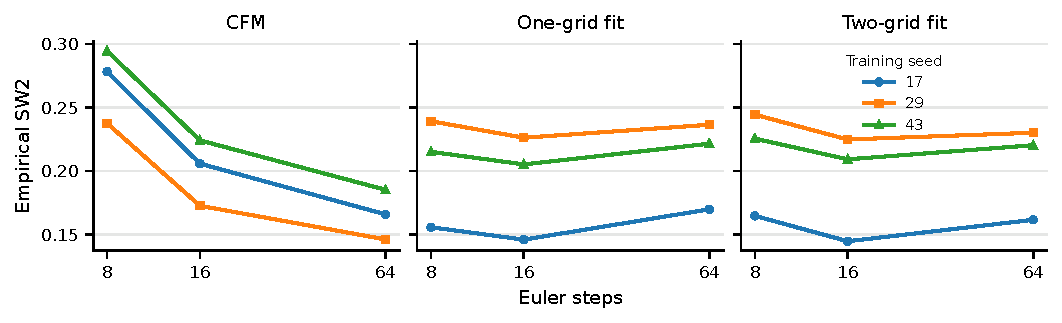
\includegraphics[width=.82\textwidth]{../results/large_bank/large_bank_d2.pdf}
\caption{Sliced Wasserstein distance (SW2) at 8, 16, and 64 Euler steps
on the 262,144-sample evaluation set. Each line is one trained field.
All nine distances decrease from 8 to 16 steps. At 64 steps, the
one-grid fields with seeds 17 and 43 have larger distances than at
8 steps.}
\label{fig:large-bank}
\end{figure}

All nine sliced distances decrease from eight to sixteen steps on this
evaluation set. Only the one-grid fields with seeds 17 and 43 increase from eight to 64 steps.
The direction of the change from 8 to 16 steps depends on the
evaluation set. The independent trigonometric
witness estimates agree with the preceding diagnostic to approximately
$5.1\times10^{-15}$. The witness metric and SW2 measure different properties of a distribution.
Their values and comparisons need not agree. They are not interchangeable
estimates of one metric.

To examine whether the shared sine/cosine form of training and diagnostic
features explains their behavior, we compare three dictionaries on the
same large evaluation set. They contain the 128 actual training features, 32
independently drawn sine/cosine features, and 32 independent functions
$\tanh(v_j^\top x-c_j)$ with $|v_j|\le1$ and $c_j\in[-2,2]$.
The last dictionary has bounded 1-Lipschitz functions and does not use
trigonometric features. We compare whether each dictionary's discrepancy increases or decreases.
The dictionaries contain different numbers and types of functions, so
their absolute values are not one common metric. For the six one-grid and two-grid fields,
both trigonometric dictionaries decrease from eight to sixteen steps.
The tanh dictionary decreases for five and increases for the one-grid field with
seed 29. Thus improvement is not confined to the shared trigonometric
form. This exploratory comparison neither establishes nor rules out a
causal training-feature preference. It adds no simultaneous confidence
claim beyond the preceding predeclared witness analysis.

\subsection{Analytical checks and global derivative bounds}
The deterministic controls check the formulas for equal refinements
$m=2,3,4$, the sharp scalar constant, degenerate splits, $N$ versus $N+1$,
equal-defect solver pairs, temporal aliasing, endpoint cancellation, and
conditional radial moments. Numerical integration checks radial moments
in selected examples. These calculations check the implementation, not the
general proof. The full inverse formula uses explicit Gaussian moments
and Hermite coefficients. Its floating-point evaluation is not an interval
certificate, and its high-degree constants can be numerically enormous.

Every fitted network has a sufficient global derivative bound established by
integer upper bounds on Frobenius norms of its exact stored binary
coefficients (Supplementary Section~\ref{app:network-budgets}). Across the 30 fitted fields,
these sufficient derivative bounds range from 12,096 to 50,688. They prove class
membership for the corresponding real tanh networks but are far too large
for a useful application of the worst-case risk thresholds. They are not
estimated local Jacobian norms or certificates for finite-precision inference.

Repetition of all 18 primary training runs in the same software environment
reproduced their parameter tensors and non-timing evaluation results.
Unit tests check finite computations; the analytical theorems rely on their
mathematical proofs.

\subsection{Population Wasserstein error on a three-dimensional mixture}
\label{app:population-example}
The target in Section~\ref{sec:population-example} is
$Y=\mu\xi e_1+\sigma Z$ with $\mu=1.5$, $\sigma=0.5$, symmetric sign
$\xi$, and independent standard Gaussian $Z$. Use the exact conditional
field \eqref{eq:mixture-generator}. In the second field, replace its
two Gaussian coordinates by the linear velocity $M'(t)M(t)^{-1}x$,
where $M(t)=(1-t)I_2+\sigma tJ$ and $J$ rotates the plane by a quarter
turn. This block has the same Gaussian marginals as the conditional
field. Its Euler update equals $M(t+h)M(t)^{-1}x$ because $M$ is affine
in time. Both fields obey a common finite derivative bound. The
mixture coordinate has the same velocity in both fields.

The exact and numerical laws each factor into a scalar law and a planar
Gaussian. Any pairing must pay at least the optimal squared cost in
each block. Since the blocks are independent, we can choose an optimal
pairing in each block and combine them. This attains the sum of the
two costs, so the squared Wasserstein distance adds across blocks.
In the plane, if the numerical and target coordinate standard deviations
are $s$ and $g(t)=\sqrt{(1-t)^2+\sigma^2t^2}$, the squared distance is
$2(s-g(t))^2$. For the skew field, this term is zero in exact arithmetic.

In the mixture coordinate, the spatial derivative of the nonlinear
velocity term is nonnegative on $[0,1]$. The spatial derivative of its linear term is
bounded below by $-(1+\sigma^2)/(2\sigma)=-1.25$. All tested Euler maps
are therefore increasing. Pair the numerical particle started from $z$
with the target point at cumulative probability $\Phi(z)$, where $\Phi$
is the standard Gaussian cumulative distribution function. This pairing
attains the scalar Wasserstein distance. Invert the two-component mixture
distribution by bisection. Integrate the squared distance against the
standard Gaussian density. Symmetry allows integration on $[0,9]$ with
twice the weight. The omitted squared tail is at most $1.07\times10^{-15}$.
To bound it, use $|X^{\mathrm{Euler}}|\le e^{1.25}(|z|+7.5)$ and the
target quantile bound $|Q_t(\Phi(z))|\le |z|+1.5$, then integrate the
square of their sum outside $[-9,9]$.

Doubling the Gauss--Legendre quadrature from 512 to 1,024 nodes changes
each reported error sum by less than $10^{-12}$ relative. The largest
relative residual in the quantile survival probabilities is below
$4\times10^{-14}$. The skew block agrees with the exact target standard
deviation within $7\times10^{-16}$. These are numerical checks on the
quadrature and floating-point arithmetic. The tail estimate is analytical.

Table~\ref{tab:population-example} gives the maxima over every shared
coarse node, separately for each run. The local order is
$\log_2(\mathcal J_{N/2}/\mathcal J_N)$. This example gives two observed
rates under the conditions of Theorem~\ref{thm:odd-transfer}. For these
fields, Theorem~\ref{thm:source-risk} also gives an obstruction. Here
$\nu=3$, and the initial excess loss $\Delta_0$ is zero for the
conditional field and $0.5$ for the skew field. Both differ from $\nu$,
so the error sum is at least of order $1/N$ for sufficiently fine grids.
Both fields generate the path exactly, so the standard Euler bound gives
an upper error of order $1/N$ on uniform grids.
The smaller error with the planar correction concerns this product path
and these two fields. The scalar optimum in Section~\ref{sec:sharpness}
concerns a different path and an optimization over fields.

\begin{table}[t]
\centering
\caption{Population $W_2$ errors for two exact generators of the three-dimensional mixture path. Errors are deterministic quadrature estimates, with no training or evaluation samples. Lower errors are better. Order is estimated from the sum of the errors at consecutive coarse step counts.}
\label{tab:population-example}
\small
\begin{tabular}{@{}r rrr rrr@{}}
\toprule
& \multicolumn{3}{c}{Conditional velocity} & \multicolumn{3}{c}{Planar skew}\\
$N$ & $E_c$ & $E_f$ & Order & $E_c$ & $E_f$ & Order\\
\midrule
8 & 0.1932745 & 0.0992033 & \multicolumn{1}{c}{--} & 0.1511015 & 0.0768981 & \multicolumn{1}{c}{--}\\
16 & 0.0992033 & 0.0503485 & 0.968 & 0.0768981 & 0.0388608 & 0.978\\
32 & 0.0503485 & 0.0253755 & 0.982 & 0.0388608 & 0.0195436 & 0.987\\
64 & 0.0253755 & 0.0127400 & 0.990 & 0.0195436 & 0.0098015 & 0.993\\
128 & 0.0127400 & 0.0063833 & 0.995 & 0.0098015 & 0.0049083 & 0.996\\
256 & 0.0063833 & 0.0031950 & 0.997 & 0.0049083 & 0.0024561 & 0.998\\
\bottomrule
\end{tabular}
\end{table}

